\newtheorem{definition}{定义}[section]
\newtheorem{example}{例}[section]
\chapter{背景知识}
\section{回答集编程}
% \numberwithin{equation}{section}
\subsection{语法}
项(terms)是ASP程序中最基本的元素,项可以是常量、变量或者函数。常量以符号常量或者数字表示(如4、a)。变量以字符串来表示,
要求首字母必须大写(如Dog、Person)。函数由函数符号与若干参数构成,例如$f(t_1,...,t_n),(n \geq 0)$。各参数
$t_i,(i=1,2,...,n)$也是项。若项中不存在函数符号与变量,则称该项为实例化项,否则称该项为非实例化项。

原子(atom)由谓词和项共同组成,例如$q(t_1,...,t_n),n \geq 0$。其中,$q$为$n$元谓词的标识符,$t_1,...,t_n$为项,
$n$为0时,谓词之后的括号可以省略。原子用于表示不同项之间的关系,例如:$dog(animal)$、$family(jensen,lucy)$、
$tomorrow\_sunny$,分别表示狗是动物、jensen和lucy是家人以及明天晴天。如果原子中的每一项都是实例化的,则该原子是实例化
原子,否则,该原子是非实例化的原子。例如,$dog(animal)$是实例化原子,$family(jensen,lucy)$是非实例化原子。
原子$q(t_1,...,t_n)$的强否定形式为$\urcorner q(t_1,...,t_)n$,其中符号$\urcorner$是经典逻辑中的否定,
$\urcorner q(t_1,...,t_n)$表示各项$t_i(1 \leq i \leq n)$。不符合
$q$所描述的关系,$\urcorner \urcorner a = a$,与经典逻辑中的排中律相同。文字(literal)可以是原子
$q(t_1,...,t_n)$,也可以是原子的强否定形式$\urcorner q(t_1,...,t_n)$。若文字对应的原子是实例化的,则称
该文字是实例化的。

\begin{definition}[规则] 规则$r$是具有如下形式的式子:
    \begin{equation}
        l_0 \thinspace or ... \thinspace or \thinspace l_m \leftarrow l_{m+1},...,l_n \thinspace not \thinspace l_{n+1},...,\thinspace not \thinspace l_p.
    \end{equation}
\end{definition}

其中$p \ge n \ge m \geq 0, l_i$代表文字,$not$为新的逻辑连接符,通常称作缺省否定符(default negation)或者
失败即否定(Negation As Failure, NAF),又称为若否定,$not \thinspace l_i$被读作“没有理由相信$l_i$为真”,但是这并不表明
$l_i$为假。对ASP程序而言,$not not a$不与a等价。规则r读作“如果相信$l_{m+1},...,l_n$为真,并且没有理由相信
$l_{m+1},...,l_p$为真,则相信$l_0 \thinspace or \thinspace ... \thinspace l_m$为真”。将$not l_i$称为缺省
文字(default literal),文字与缺省文字共同组成拓展文字(extended literal)。

规则$r$左侧的文字称为头部,可以表示为$head(r) = \{ l_0,...,l_m \}$。规则$r$右侧的文字称为体部,可以表示为
$body(r) = \{ l_{m+1},...l_n,not \thinspace l_{n+1},..., not \thinspace l_p \}$,规则的体部可以分为正
体部与负体部,正体部表示为$body^+(r) = \{ l_{m+1},...,l_n \}$,负体部表示为$body^-(r)=\{ l_{n+1},...,l_p \}$
。因此,规则$r$可以表示为:
\begin{equation}
    head(r) \thinspace \leftarrow \thinspace body^+(r), \thinspace not body^-(r) \label{con:body}
\end{equation}
一个ASP程序是有限条\eqref{con:body}所示的规则组成的集合。根据规则各部分所满足的相关条
件,可以分别定义事实、约束、正规规则、缺省规则和严格规则,如定义\eqref{def:fact}-定义\eqref{def:definite_rule}所
示。

\begin{definition}[事实]
当规则$r$满足$head(r)\neq \emptyset, body(r) = \emptyset$时,被称为事实(fact)。\label{def:fact}
\end{definition}
\begin{definition}[约束]
当规则$r$满足$head(r)= \emptyset, body(r) \neq \emptyset$时,被称为约束(constraint)。
\end{definition}
\begin{definition}[正则规则]
    当规则$r$满足$|head(r)|=1$时,被称为正则规则(normal rule)。
\end{definition}
\begin{definition}[缺省规则]
    当规则$r$满足$body(r)^-\neq \emptyset$时,被称为缺省规则(default rule)。
\end{definition}
\begin{definition}[严格规则]
    当规则$r$满足$body(r)^- = \emptyset$时,被称为严格规则(definite rule)。\label{def:definite_rule}
\end{definition}
根据上述各类规则的定义,本文进一步定义简单逻辑程序、缺省逻辑程序和正规逻辑程序如下。
\begin{definition}[简单逻辑程序]
    若程序$P$由有限条严格规则组成,则$P$被称为简单逻辑程序。
\end{definition}
\begin{definition}[拓展逻辑程序]
    若程序$P$由有限条缺省规则组成,则$P$被称为拓展逻辑程序。
\end{definition}
\begin{definition}[正则逻辑程序]
    若程序$P$除约束外,由有限条正则规则组成,则$P$被称为正则逻辑程序(Normal Logic Program, NLP)。
\end{definition}
若不做特别说明,本文考虑的程序均为不含约束的正规逻辑程序,即程序中的每条规则头部有且仅有一个文字。
\subsection{语义}
\subsubsection{文字的可满足性语义解释和程序的模型}
作为基础理论,首先给出 Herbrand 域、Herbrand 基的定义,分别如定义2.10和2.11所
示,进一步定义规则与程序的实例化,最终在实例化程序下讨论文字的可满足性语义解
释和可满足性。
\begin{definition}[Herbrand基]
    $P$是一个 ASP 程序,将程序$P$中出现的常量和函数形成的
    所有不含变量的项的集合称为 Herbrand 域,使用$\mathcal{U}_P$表示。
\end{definition}
\begin{definition}[Herbrand域]
    $P$是一个 ASP 程序,出现在程序$P$的规则中的谓词符号与
$\mathcal{U}_P$中的项组成的所有可能的不含变量的原子集合称为程序$P$的 Herbrand 基,使用$\mathcal{A}_P$
表示,为了保持简洁,通常简写为$\mathcal{A}$。
\end{definition}
\begin{definition}[规则的实例化]
    给定$P$中的一个规则$r$,使用$ground(r)$表示通过使用
$\mathcal{A}_P$中的常量对应地替换$r$中变量而获得的规则集合,这一映射被称为规则的实例化。
\end{definition}
\begin{definition}[程序的实例化]
    程序$P$由一系列规则的集合组成,程序$P$的实例化$ground(P)$表示为式\eqref{equation:ground}:
    \begin{equation}
    ground(P)=\bigcup_{r \in P}ground(r) \label{equation:ground}
    \end{equation}
\end{definition}
\begin{definition}[文字的可满足性语义解释]
    定义文字的可满足性语义解释$I=\langle I^+,I^- \rangle$,其中$I^+\cup I^-\subseteq \mathcal{A}_P$
    ($P$是实例化程序),$I^+\cap I^-=\emptyset$。$I^+$表示为已知为真的文字集合,$I^-$表示已知为假
    的文字集合。当$I^+\cap I^-=\mathcal{A}_P$时,$I$被称作完全可满足性语义解释(complete interpretation)。
    若I不是完全可满足性语义解释,则$I$中存在真值未确定(undefined)的文字。
\end{definition}
\begin{definition}[程序的模型]
    假设$P$是一个实例化的回答集程序,$I=\langle I^+,I^- \rangle$是一个可满足性语义解释。若文字$l \in I^+$,
    则称I满足$l$,记作$I\models l$;对缺省文字$not l$,若$l \in I^-$,则称I满足$not l$,记作$I\models not l$。
    对于文字集合$S$,若$\veebar l \in S,I \models l$,则称$I$满足集合$S$,记作$I \models S$,当一个规则
    $r$满足$I \nvDash body(r)$或$I \models head(r)$时,$I$满足规则$r$。当$I$满足程序$P$的所有规则时,称
    $I$是$P$的一个模型。
\end{definition}
\subsubsection{回答集语义}
\begin{definition}[一致性文字集合]
    给定一个文字集合$S$,若$S$中不同时包含$l$和$\urcorner l$,则集合S是一致性文字集合,其中,$l \in S$是集合
    S中的任意文字。
\end{definition}
\begin{definition}[可满足性,Satisfiability]
    给定一致性文字集合$S$,文字$lit$与规则 $r$,若
$lit \in S$,则文字$ lit $满足集合 $S$。若 $head(r)\cap S \neq \emptyset$,则 $S $满足头部。若$ body^+(r) \subseteq 
S, S ∩ body^−(r) = \emptyset$,则集合$ S $满足体部。若 $S $满足规则 $r$ 的头部或者 $S $不满足规则$ r$ 的
体部,则$ S$满足规则 $r$,记作$ S \models r$。给定一个 ASP 程序 $P$,若 $\veebar r \in P, S \models r$,则 $S$ 满足
程序 $P$。
\end{definition}
\begin{definition}[规则的适用与阻塞]
    给定一致性文字集合 $S$ 与规则 $r$,$S$ 满足 $body(r)$,
则称规则 $r $在集合$S $下是适用的(applicable),否则称规则$ r $在集合$ S$ 下被阻塞(block)。
\end{definition}
\begin{example}
    给定ASP程序$P_3$,该程序包含两条规则:
    \begin{align*}
        &r_1: p \leftarrow q, s. \\ 
        &r_2: s \leftarrow t.
    \end{align*}
\end{example}
下面通过分析说明集合$S=\{ p, q\}$对程序$P$的可满足性。
\begin{enumerate}[label=(\arabic*),itemsep=0pt,parsep=0pt]
    \item 因为$p\in S$,所以文字$p$与文字$q$均满足$S$;
    \item 因为$S \cap head(r_1) = \{ p \} \neq \emptyset$,所以$S$满足$head(r_1), S \models r_1$;
    \item 因为$body^+(r_2) \subsetneq S$,所以$S$不满足$body(r_2)$,所以$S \models r_2$;
    \item 因为$S$满足程序$P$中的每一条规则,所以$S$满足程序$P$。
\end{enumerate}
\begin{definition}[Gelfond-Lifshitz规则(GL规约)]
    假设程序 $P$ 是给定的实例化程序,$S$
是一致性文字集合,$l$ 是文字,$S \subseteq  Lit(P), l \in Lit(P)$, $P $关于 $S$ 的$ GL$ 规约结果$ P^S$定义为式\eqref{equation:GL}:
\begin{equation}
    P^S = \{ head(r) \leftarrow body^+(r) \mid r \in P, body^-(r) \cap S = \emptyset \} \label{equation:GL}
\end{equation}
\end{definition}
\begin{definition}[简单逻辑程序回答集\cite{}]
    假设$P$是简单逻辑程序,程序$P$的回答集是$S \subseteq Lit(P)$ 满足:

    \begin{enumerate}[label=(\arabic*),itemsep=0pt,parsep=0pt]
        \item 对于程序$P$中的每一条规则$l_0 \leftarrow l_1,...,l_m$,如果$l_1,...,l_m \in S$,那么$l_0 \in S$。
        \item $S \subseteq Lit(P)$且不存在$ S$ 的任何子集也满足程序 $P$ 的每一个规则,即 $S $是满足程序$ P$的最小集合;
        \item 如果 $S$ 包含互补的文字,那么 $S = Lit(P)$;
    \end{enumerate}
\end{definition}
\begin{definition}[拓展逻辑程序回答集]
    假设$P$是包含缺省否定的扩展逻辑程序,$S$是实例化文字集合,如果$S$是$P^S$的回答集,则$S$是$P$的回答集。如果程序$P$没有回答集或
者只有一个包含互补文字的回答集$Lit(P)$,那么程序$P$是不一致程序,否则,程序$P$是一致性程序。

可以看出,使用 GL 规约,可以将扩展逻辑程序程序转换为简单逻辑程序,从而得到扩展逻辑程序的回答集。下面通过一个例子说明。
\begin{example}[GL规约与问答集]
    给定一个实例化的ASP程序$P_4$:
    \begin{align*}
        &r_1: p(a) \leftarrow not p(b) \\
        &r_2: p(b) \leftarrow not p(a) \\
        &r_3: \leftarrow p(b).
    \end{align*}
    程序$P_4$可能的回答集有四个:$S_1 = \emptyset, S_2 = \{ p(a) \}, S_3 = \{ p(b) \}, S_4 = 
    \{ p(a), p(b) \}$, 根据回答集的定义依次验证:
    \begin{enumerate}[label=(\arabic*),itemsep=0pt,parsep=0pt]
        \item $P^{S_1} = \{ p(a) \leftarrow .\} \cup \{ p(b) \leftarrow . \} \cup \{ \leftarrow p(b) .\}$,事实$(p(b) \leftarrow .)$
    与约束$(\leftarrow p(b).)$同时在$P^{S_1}$中出现,因此$S_1$不是$P^{S_1}$的回答集,所以$S_1$不是$P$的回答集。
        \item $P^{S_2} = \{ p(a) \leftarrow .\} \cup \{ \leftarrow p(b) .\}$,而$S_2 \models ((p(a) \leftarrow .))$且
    $S_2 \models (\leftarrow p(b).)$,因此$S_2 \models P^{S_2}$,且不存在$S_2^{'}\subset S_2, S_2^{'} \models P^{S_2}$,所以$S_2$是$P^{S_2}$的回答集;

        \item $P^{S_3} = \{ p(b) \leftarrow . \} \cup \{ \leftarrow p(b) .\}$,事实$(p(b) \leftarrow .)$
    与约束$(\leftarrow p(b).)$同时在$P^{S_3}$中出现,因此$S_3$不是$P^{S_3}$的回答集,所以$S_3$不是$P$的回答集;
        \item $P^{S_4} = \{ \leftarrow p(b). \}$,可知$P^{S_4}$的回答集为$\emptyset$,因此$S_4$不是
    $P^{S_4}$的回答集,所以$S_4$不是$P$的回答集。
    \end{enumerate}
\end{example}
\end{definition}

\subsubsection{well-founded语义}
上世纪 90 年代,良基语义(well-founded semantics)的概念由 Van Gelder A 提出,
对于任意的回答集程序,都存在对应的良基模型(well-founded models),并且在多项式
时间内可以计算出这个模型\cite{van1991well}。该语义模型是本文对 NAF 文字进行解释和对不一致程
序原因进行分类的重要基础,下面介绍这一模型的定义及计算方法。

\begin{definition}[立即结论]
$P$是一个 ASP 程序,$S\subseteq \mathcal{A}_P,V\subseteq \mathcal{A}_P$,则集合$S$关于$P$和$V$的
立即结论(immediate consequence)记作 $\mathcal{T}_{P,V}(S)$,定义如式\eqref{equation:immediate_consequence}所示:
\begin{equation}
    T_{P,V}(S) = \{ a | \exists r \in P, head(r) = a, body^+(r) \subseteq S, body^-(r)\cap V = \emptyset \} \label{equation:immediate_consequence}
\end{equation}
\end{definition}
考察上式可以发现,当集合$V$确定时,关于集合$S$的函数$T_{P,V}(S)$是单调的。因此,当集合$V$固定时,该函数
存在最小不动点(Least Fixed Point, LFP),使用$lfp(.)$表示。

\begin{definition}[良基模型]
    $P$是一个 ASP 程序,$P^+$是程序$P$中的全部严格规则的集合,序列$(K_i,U_i)_{i \geq 0}$定义如下:
    \begin{align*}
        &K_0 = \mathit{lfp}(T_{P^+}) & K_i &= \mathit{lfp}(T_P, U_{i-1}) \\
        &U_0 = \mathit{lfp}(T_{P, K_0}) & U_i &= \mathit{lfp}(T_{P, K_i})
    \end{align*}
\end{definition}
若$\langle K_j,U_j \rangle = \langle K_{j+1},U_{j+1} \rangle$,且不存在$0 \leq k < j$,使得
$\langle K_k, U_k = \langle K_{k+1},U_{k+1} \rangle$(j,k是正整数),则$P$的良基模型$WF_P=\langle W^+,W^- \rangle$,
满足$W^+=K_j$,$W^-=\mathcal{A}\backslash U_j$
\begin{example}[良基模型]
    程序$P_5$包含以下四条规则:
    \begin{align*}
        &r_1:q \leftarrow , not p. &r_2: p \leftarrow, not q. \\
        &r_3:a \leftarrow b. &r_4: b \leftarrow. 
    \end{align*}
\end{example}
首先得到$P_5^+=\{ a \leftarrow b \} \cup \{b \leftarrow . \}$,而$lfp(T_{P_5^+}) = {a, b}$,因此
$K_0 = {a,b}$;进一步计算得到$U_0 = lfp(T_{P_5^+, K_0}) = \{ a,b,p,q \}$,$K_1 = lfp(T_{P_5^+, U_0}) = 
\{ a, b \} = K_0$,$U_1 = lfp(T_{P_5^+,K_1}) = \{ a,b,p,q \} = U_0$。因此$\langle K_0, U_0 \rangle = 
\langle K_1, U_1 \rangle$且不存在$0 \leq k < 1$,$\langle K_k, U_k \rangle = \langle K_{k+1}, U_{k+1} \rangle$。
因此程序$P_5^+$的良基模型为$WF_{P_5^+} = \langle \{a, b\}, \{ \} \rangle$,$p$和$q$在良基模型中属于
未定义($undefined$)。
\subsection{求解器}
求解器是实现ASP语义推理的核心工具,其工作原理是:通过搜索逻辑程序的最小模型(即回答集)来解决复杂的组合优化问题。

求解器的工作流程可以划分为两个阶段:基础化(Grounding)和求解(Solving)。
基础化是将一阶逻辑程序实例化为命题逻辑形式,而求解则是基于CDCL算法搜索满足约束的模型。

截至目前,已经有众多ASP求解器。学术界和工业界所用的主流的求解器,可分为两类:单阶段求解器(如Clasp、DLV)、
多阶段求解器(如Clingo)。两类求解器的主要区别在于,单阶段求解器独立地进行基础化与求解,而多阶段求解器
则是集成了基础化与求解的交互式系统。

表\ref{tab:solver_comparison}对目前的主流求解器的适用场景及核心优势进行了对比。因为 Clingo 求解器
具有免费开源、使用简单、运行高效的特点,本文在求解 ASP程序时,使用 Clingo 进行相关实验。
\begin{table}[h]
    \centering
    \renewcommand{\arraystretch}{1.2} % 增加行距,避免分割线和文本重叠
    \begin{tabular}{l l l l}
        \toprule
        \textbf{求解器} & \textbf{核心技术} & \textbf{适用场景} & \textbf{核心优势} \\
        \midrule
        Clasp  & \multirow{2}{*}{\hspace{0.5em} 多线程CDCL} & \multirow{2}{*}{\hspace{0.5em} 大规模组合优化} & \multirow{2}{*}{\hspace{0.5em} 支持并行搜索} \\
               & \multirow{2}{*}{\hspace{0.5em} 情性子句学习} & \multirow{2}{*}{\hspace{0.5em} 工业级应用} & \multirow{2}{*}{\hspace{0.5em} 性能竞赛冠军} \\
        \midrule
        Clingo & \multirow{2}{*}{\hspace{0.5em} 增量式基础化} & \multirow{2}{*}{\hspace{0.5em} 动态规则生成} & \multirow{2}{*}{\hspace{0.5em} 集成Python API} \\
               & \multirow{2}{*}{\hspace{0.5em} 多阶段编程} & \multirow{2}{*}{\hspace{0.5em} 交互式推理} & \multirow{2}{*}{\hspace{0.5em} 支持在线更新程序} \\
        \midrule
        DLV    & \multirow{2}{*}{\hspace{0.5em} 数据库优化} & \multirow{2}{*}{\hspace{0.5em} 知识表示型问题} & \multirow{2}{*}{\hspace{0.5em} 高效处理复杂规则} \\
               & \multirow{2}{*}{\hspace{0.5em} 存在线量化推理} & \multirow{2}{*}{\hspace{0.5em} 语义Web} & \multirow{2}{*}{\hspace{0.5em} 支持非确定域} \\
        \midrule
        WASP   & \multirow{2}{*}{\hspace{0.5em} 分层弱约束优化} & \multirow{2}{*}{\hspace{0.5em} 偏好推理} & \multirow{2}{*}{\hspace{0.5em} 加权约束高效处理} \\
               & \multirow{2}{*}{\hspace{0.5em} 冲突驱动剪枝} & \multirow{2}{*}{\hspace{0.5em} 多目标优化} & \\
        \midrule
        Smodels & \multirow{2}{*}{\hspace{0.5em} 稳定模型算法} & \multirow{2}{*}{\hspace{0.5em} 教学与研究} & \multirow{2}{*}{\hspace{0.5em} 算法透明易扩展} \\
                & \multirow{2}{*}{\hspace{0.5em} 部分求值} & \multirow{2}{*}{\hspace{0.5em} 基础模型验证} & \\
        \midrule
        LPARSE  & \hspace{0.5em} 基础化预处理 & \hspace{0.5em} 规则实例优化 & \hspace{0.5em} 与Smodels配合使用 \\
        \midrule
        IDP    & \multirow{2}{*}{\hspace{0.5em} 基于模型的推理} & \multirow{2}{*}{\hspace{0.5em} 复杂知识库管理} & \multirow{2}{*}{\hspace{0.5em} 支持类型系统} \\
               & \multirow{2}{*}{\hspace{0.5em} 扩展一阶逻辑} &  & \multirow{2}{*}{\hspace{0.5em} 高阶推理} \\
        \midrule
        Alpha  & \hspace{0.5em} 并行求解引擎 & \hspace{0.5em} 超大规模问题 & \hspace{0.5em} GPU加速搜索 \\
        \bottomrule
    \end{tabular}
    \caption{扩展后的系统对比}
    \label{tab:solver_comparison}
\end{table}

\section{GLIP}
GLIP(Grounded Language-Image Pretraining)是一种融合视觉与语言的预训练模型,旨在提高模型在目标检测、图像理解以及跨模态任务上的能力。GLIP 通过对大规模的图像-文本对数据进行联合训练,使得模型能够理解自然语言查询,并在图像中定位相应的目标,从而实现零样本(zero-shot)或少样本(few-shot)的目标检测任务。
其架构如图\ref{GLIP_architecture}所示。

GLIP采用了大规模的图像-文本数据进行预训练,使用基于 Transformer 的架构,并结合视觉和语言的特征进行跨模态学习。其训练过程主要包括:
(1)文本引导的目标检测:输入不仅包含图像,还包含文本描述,使得模型能够基于自然语言查询来识别目标。
(2)跨模态对齐:通过对比学习和注意力机制,使得视觉特征与语言特征在共享的表示空间中进行对齐。
(3)自监督学习:利用大规模无标注数据进行自监督学习,提高模型的鲁棒性和泛化能力。

相比以往的目标检测技术,GLIP的突出优势在于:
(1)零样本检测能力:无需重新训练,即可识别新的类别。
(2)泛化性强:由于使用了开放词汇的文本描述,GLIP 在实际应用中更加灵活。
(3)跨领域适应性:可以应用于医学影像分析、自动驾驶、机器人视觉等多个领域。

目前,GLIP在多个计算机视觉任务中表现优异,典型的应用包括:开放词汇目标检测(Open Vocabulary Object Detection, OVOD)、
跨模态信息检索、复杂视觉问答(Visual Question Answering, VQA)、自动标注和数据增强。

\begin{figure}
    \centering
    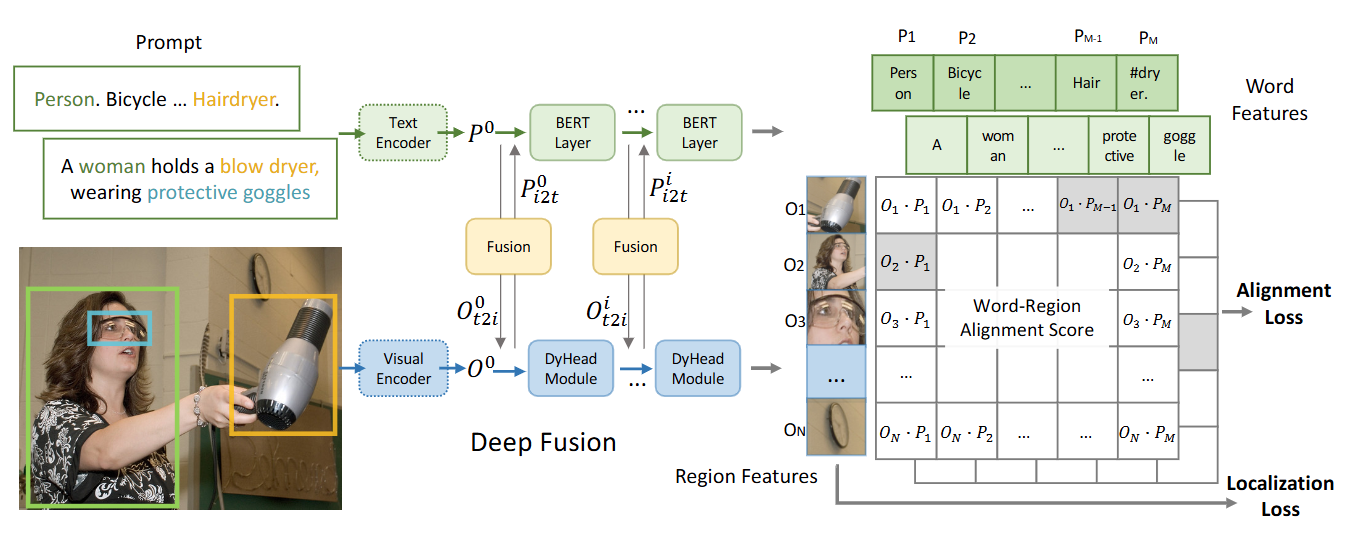
\includegraphics[width=\textwidth]{GLIP_architecture.jpg}
    \caption{GLIP结构示意图\label{GLIP_architecture}}
\end{figure}

\section{大语言模型}

\section{DSPy}
DSPy(Declarative Self-improving Language Programs)是由斯坦福大学开发的一种编程框架,旨在通过声明式的方式优化大语言模型(LLMs)的推理能力。DSPy 提供了一种高效的途径,使开发者能够构建自我改进的自然语言处理(NLP)系统,而无需手动调整复杂的超参数或微调大模型。

DSPy 的核心思想是将模型的优化过程抽象为声明式编程,使得用户能够专注于高层任务,而底层优化(如提示工程、少样本学习等)由系统自动完成。其主要特性包括:
(1)模块化设计:开发者可以定义不同的语言任务模块,DSPy 会自动优化这些模块的执行方式。
(2)自适应优化:系统会根据反馈数据不断调整推理策略,提高模型的准确性和鲁棒性。
(3)多模态支持:除了纯文本处理,DSPy 还可以用于多模态任务,如结合视觉和语言进行推理。

DSPy 采用了多种技术来提高大语言模型的推理效率和准确性,包括:
(1)自动提示调整(Auto-Prompting):根据任务需求,动态优化提示词,提高模型的响应质量。
(2)少样本学习(Few-shot Learning):利用少量示例进行任务适配,减少对大规模标注数据的依赖。
(3)强化学习(Reinforcement Learning):通过用户反馈不断优化推理过程,使模型的输出更加符合期望。

使用DSPy构建大语言模型应用,具有如下优势:
(1)声明式编程范式:减少了对低层次参数调整的需求,使开发者可以更专注于任务逻辑。
(2)高效优化:通过自动调整提示词和推理策略,提高大模型的推理能力。
(3)可扩展性强:适用于各种NLP任务,包括文本摘要、信息抽取、代码生成等。

\section{本章小结}